\documentclass[11pt,letterpaper]{article}
\usepackage[margin=1in]{geometry}
\usepackage{graphicx}
\usepackage{hyperref}
\usepackage{listings}
\pagestyle{headings}
\usepackage{epstopdf}

\begin{document}

\title{PHY 410 \\ Homework Assignment 4}
\author{Han Wen \\ \tiny Person No. 50096432}
\date{\today}

\maketitle

\begin{abstract}
The goal of this assignment was to develop a thorough understanding of Integral and root finding as well as the classical scattering problem
\end{abstract}

\tableofcontents

\newpage
\section{Problem 1}

\subsection{Description}
Compare the accuracies and efficiencies of any two quadrature algorithms on the definite integral:
$$
\int_0^1 e^x\mathrm{d}s=e-1
$$
Compare the accuracies and convergence rates of any two root-finding algorithms on the functions:
$$
f(x)=tan(x),   f(x)=tanh(x)
$$



\subsection{Solution}
For part one, I used both Trapezoidal rule and Simpson rule to do the integral. And generated a plot of accuracies vs. number of the steps used. ~\ref{figure1}
Apparently using simpson gives much higher accuracy. Considering they both used same number of summations during the procedure. Therefore the simpson is more effective. 


For part two. I used both simple search and root tangent method. First from basic knowledge we know for tan function periodic roots occur while for tanh the only root is the origin point. For simplicity I am going to test only the origin point root.\\
$tan$:\\
	Simple search:\\		initial guess:-1\\		initial step: 0.3 \\		accuracy: 0.0000001.\\
	It takes 35 steps to find the root, and the function value is $4.77\times10^{-8}$.
	\\
	Root tangent:\\		initial guess:-1\\		accuracy:0.0000001\\
	It takes 4 steps to find the root, the function value is $-2.32\times10^{-10}$\\

$tanh$:\\	Simple search:\\		initial guess:-1\\   initial step: 0.3\\		accuracy: 0.0000001\\
	It takes 35 steps to find the root, and the function value is $4.77\times10^{-8}$\\
	Root tangent:\\		initial guess:-1\\		accuracy:0.0000001\\
	It takes 5 steps to find the root, the function value is $2.34\times10^{-13}$
\\\\
Therefore we can see the root tangent method gives faster convergence rates and better accuracy.

\begin{figure}
\begin{center}
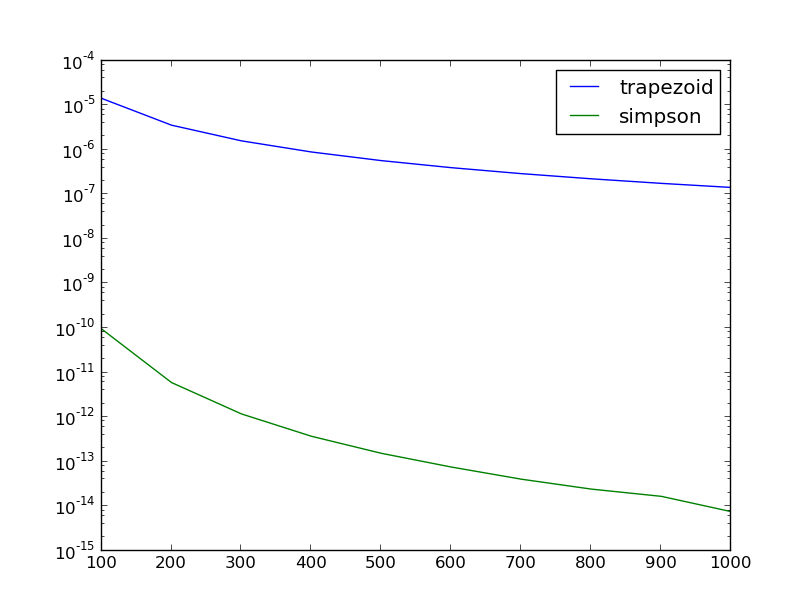
\includegraphics[width=0.9\linewidth,angle=0]{p1accuracy.png}
\caption{accuracies vs. number of the steps used, problem 1}
\label{figure1}
\end{center}
\end{figure}


\section{Problem 2}

\subsection{Description}

Using the tools from Lecture 12, study classical scattering from a hard sphere and from the Lennard-Jones potential. As discussed in Lecture 12, plot typical trajectories, and compute and plot the differential scattering cross section for the Lennard-Jones case (as per the procedure from class, Slide 16 in Lecture 12). Do this for two or three different values of the energy that you find most interesting. Study the phenomenon of orbiting in the Lennard-Jones case: what is the maximum number of orbits you can generate by carefully tuning the energy and impact parameter?

\subsection{Result}
Here is the plot of the trajectories of hard-core potential for various d with E=0.705 ~\ref{figure2}.\\
Here is the plot of the trajectories of Lennard-Jones potential for various d with E=0.705 ~\ref{figure3}.\\
Here is the plot of differential cross section vs. d for Lennard-Jones potential with E=0.705 ~\ref{figure4}.\\


\begin{figure}
\begin{center}
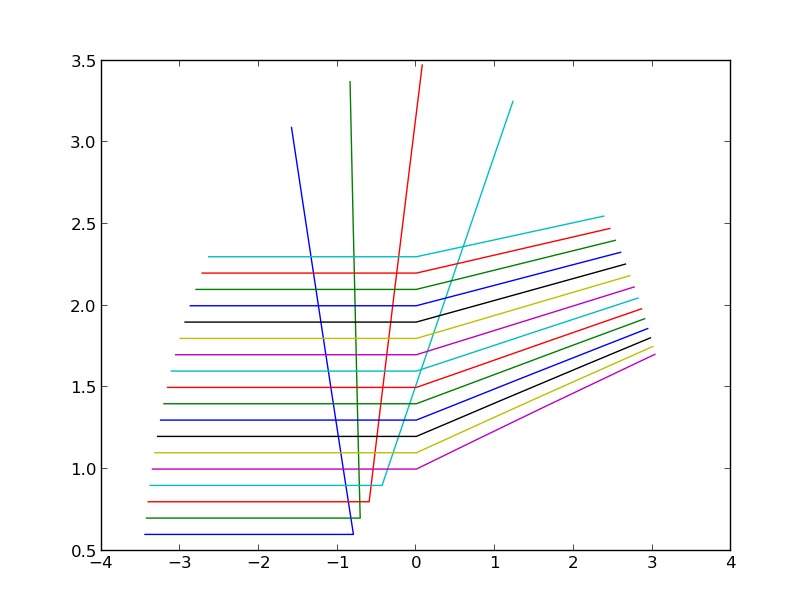
\includegraphics[width=0.9\linewidth,angle=0]{p2allhard.png}
\caption{Hard core trajectories with various d, E=0.705}
\label{figure2}
\end{center}
\end{figure}


\begin{figure}
\begin{center}
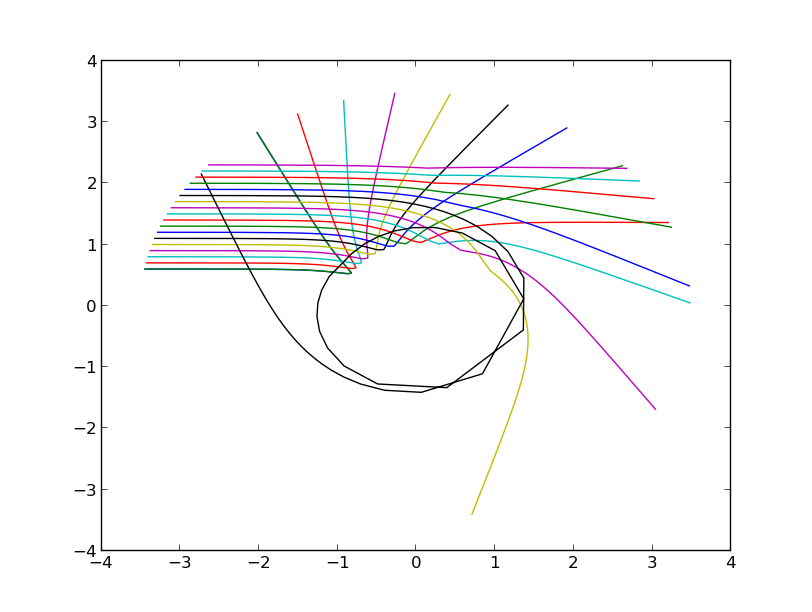
\includegraphics[width=0.9\linewidth,angle=0]{p2alldtra.png}
\caption{Lennard-Jones trajectories with various d, E=0.705}
\label{figure3}
\end{center}
\end{figure}

\begin{figure}
\begin{center}
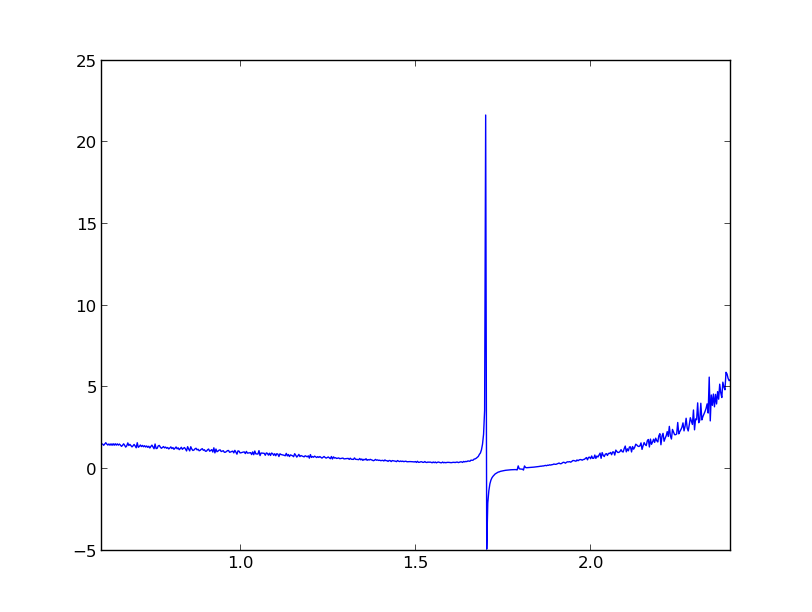
\includegraphics[width=0.9\linewidth,angle=0]{p2diffE0705.png}
\caption{Lennard-Jones differential cross section vs. d, E=0.705}
\label{figure4}
\end{center}
\end{figure}




Here is the plot of the trajectories of hard-core potential for various d with E=1.705 ~\ref{figure5}.\\
Here is the plot of the trajectories of Lennard-Jones potential for various d with E=1.705 ~\ref{figure6}.\\
Here is the plot of differential cross section vs. d for Lennard-Jones potential with E=1.705 ~\ref{figure7}.\\


\begin{figure}
\begin{center}
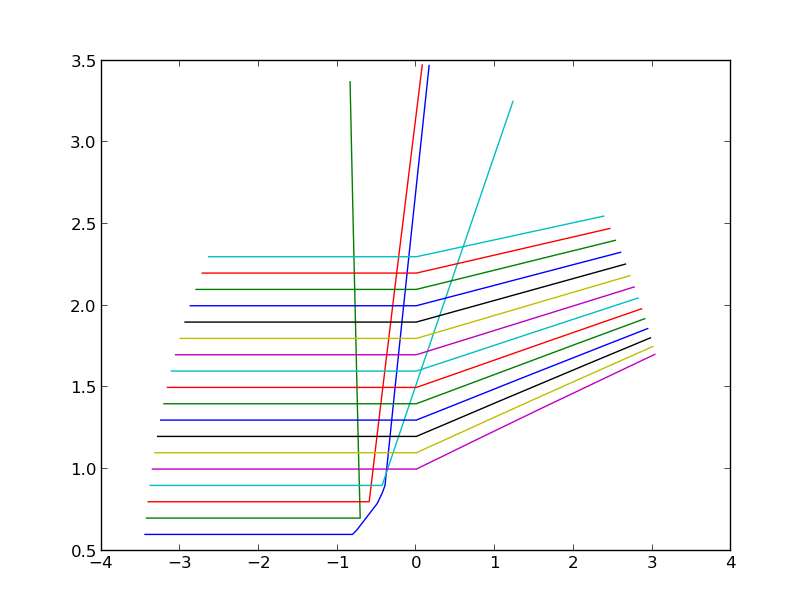
\includegraphics[width=0.9\linewidth,angle=0]{p2allhard1715.png}
\caption{Hard core trajectories with various d, E=1.705}
\label{figure5}
\end{center}
\end{figure}


\begin{figure}
\begin{center}
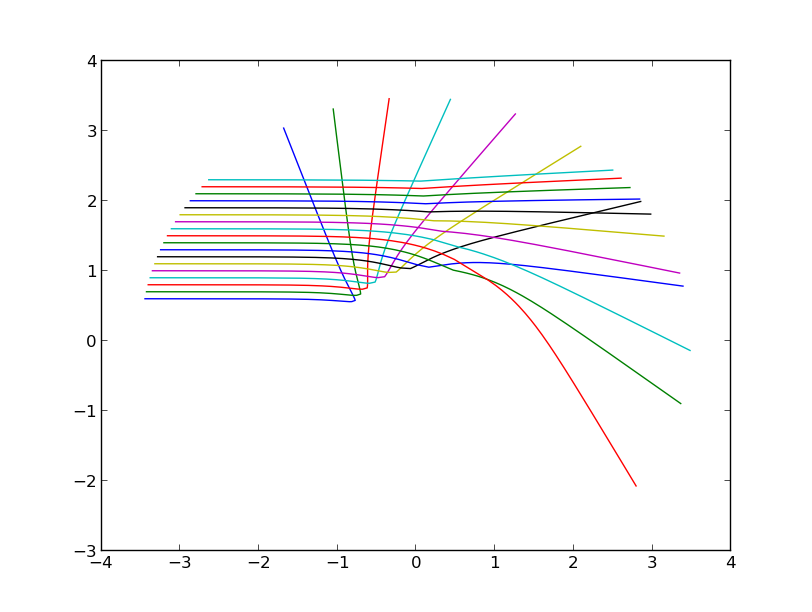
\includegraphics[width=0.9\linewidth,angle=0]{p2alldtra1715.png}
\caption{Lennard-Jones trajectories with various d, E=1.705}
\label{figure6}
\end{center}
\end{figure}

\begin{figure}
\begin{center}
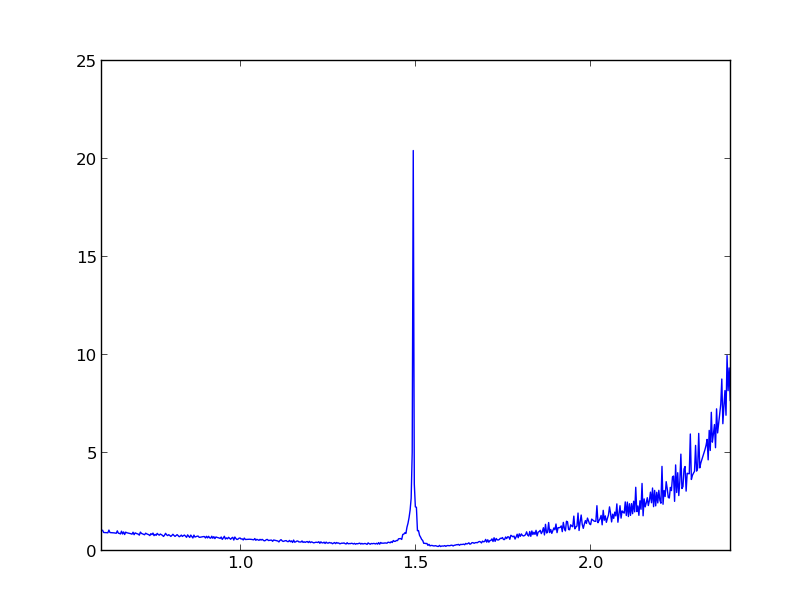
\includegraphics[width=0.9\linewidth,angle=0]{p2diffE1705.png}
\caption{Lennard-Jones differential cross section vs. d, E=1.705}
\label{figure7}
\end{center}
\end{figure}


Here is the plot of the trajectories of hard-core potential for various d with E=2.705 ~\ref{figure8}.\\
Here is the plot of the trajectories of Lennard-Jones potential for various d with E=2.705 ~\ref{figure9}.\\
Here is the plot of differential cross section vs. d for Lennard-Jones potential with E=2.705 ~\ref{figure10}.\\


\begin{figure}
\begin{center}
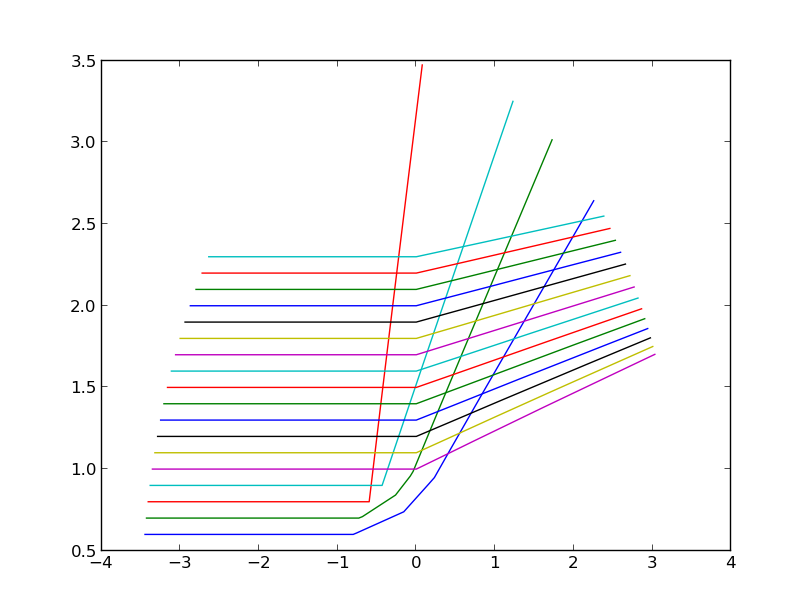
\includegraphics[width=0.9\linewidth,angle=0]{p2allhard2715.png}
\caption{Hard core trajectories with various d, E=2.705}
\label{figure8}
\end{center}
\end{figure}


\begin{figure}
\begin{center}
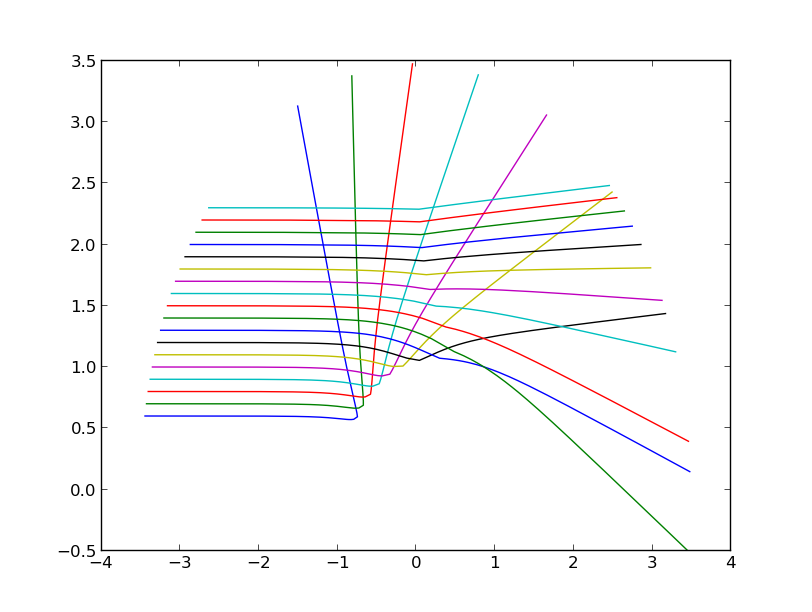
\includegraphics[width=0.9\linewidth,angle=0]{p2alldtra2715.png}
\caption{Lennard-Jones trajectories with various d, E=2.705}
\label{figure9}
\end{center}
\end{figure}

\begin{figure}
\begin{center}
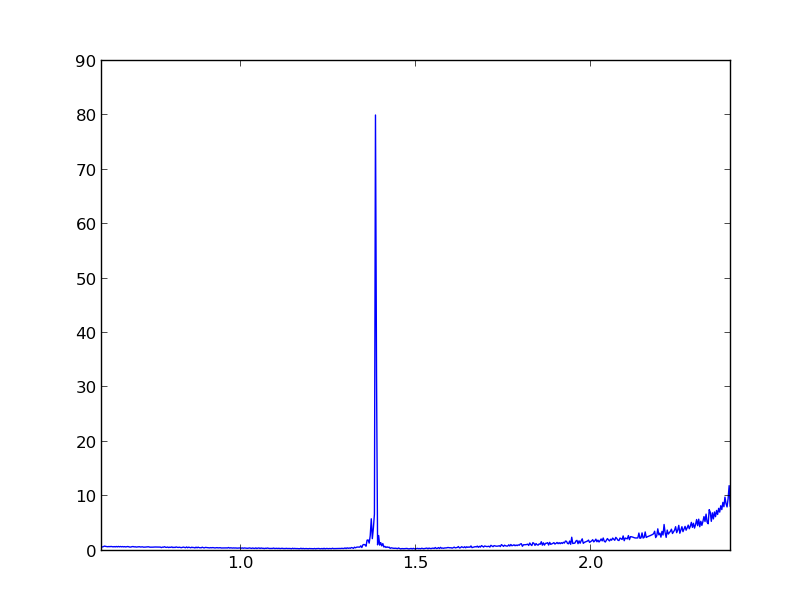
\includegraphics[width=0.9\linewidth,angle=0]{p2diffE2705.png}
\caption{Lennard-Jones differential cross section vs. d, E=2.705}
\label{figure10}
\end{center}
\end{figure}

\newpage

\section{Problem 3}
\subsection{Description}
(a) Show that the tangent root-finding algorithm is unstable for starting   bigger than a critical value in Problem 1, and find this value. (b) Modify the scattering program to plot trajectories and differential cross sections for the screened Coulomb or Yukawa potential
$$
V(r)=V_0\frac{e^{-r/r_0}}{r}
$$

Compare your results in the limit of large $r_0$ with analytic formulas for Rutherford scattering (as derived in class).
\subsection{Result}
(a) From the algorithm we can see the reason of existence of the unstable guess is that some value will make the first derivative of the function approach to 0, especially when it thus will cause the value of the first derivative in the next step more approach to 0. In our case, the first function is fine, there will be no so called critical value. Yet for the hyperbolic tangent. We can see for x goes to infinity, the value of tanh(x) goes to plus or minus 1, resulting in its first derivative approaching 0. With an accuracy of 0.0000001, the critical value is about 1.08.   
\\
(b)Using the Yukawa potential with E=0.705 and $r_0=1.0$, I plot the trajectories of various d: ~\ref{figure11}, and differential cross section vs. d ~\ref{figure12}

\begin{figure}
\begin{center}
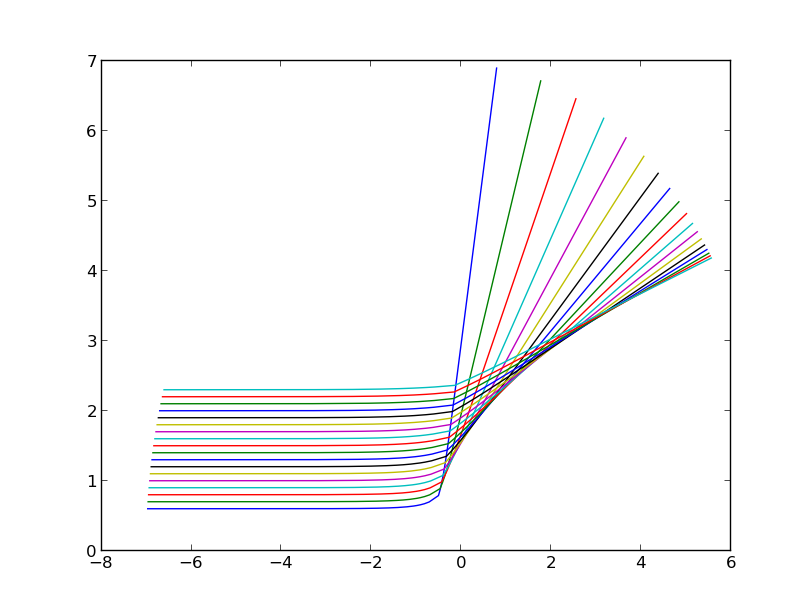
\includegraphics[width=0.9\linewidth,angle=0]{Yukawaall.png}
\caption{Yukawa trajectories with various d, E=0.705}
\label{figure11}
\end{center}
\end{figure}

\begin{figure}
\begin{center}
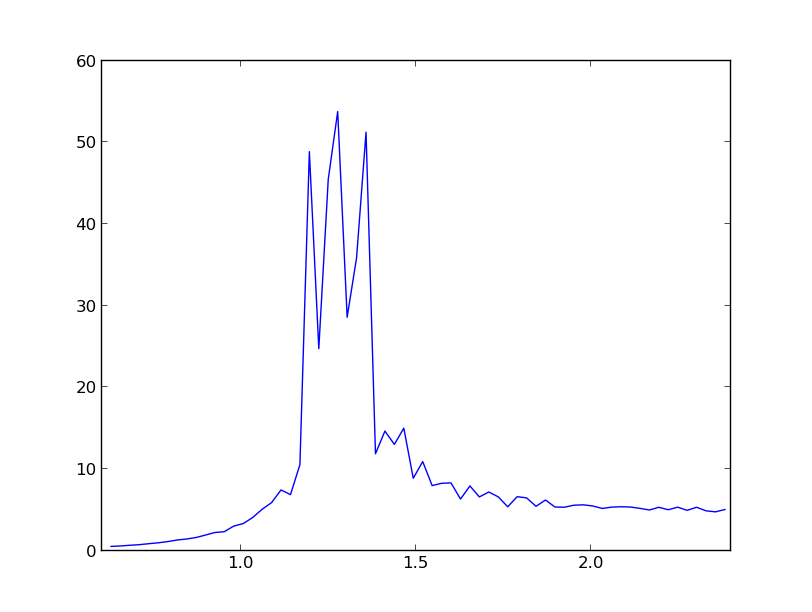
\includegraphics[width=0.9\linewidth,angle=0]{Yukawad.png}
\caption{Yukawa differential cross section vs. d, E=0.705}
\label{figure12}
\end{center}
\end{figure}


When $r_0$ is becoming very large, from the analytical point of vies, the Yukawa potential scattering will general approach Rutherford scattering. 
However here is a little comments about what we discussed in the afternoon. When talking about the big $r_0$ behaviour you quoted wikipedia \url{http://en.wikipedia.org/wiki/Rutherford_scattering}. However, you mistook the b below as the b in the equation, while in fact that b is the nearest location, not related to scattering. The real d is a function of $\Theta$, and thus the $\frac{d\sigma}{d\Omega}$ is not purely a function of $d^2$ unless when d is quite big where the $\Theta$ does not change too much with d, at which time approximately the square rule can apply. And my simulation verified my theory:
Here is the diagram when d starts from a rather big value with $r_0=10$: ~\ref{figure13}


\begin{figure}
\begin{center}
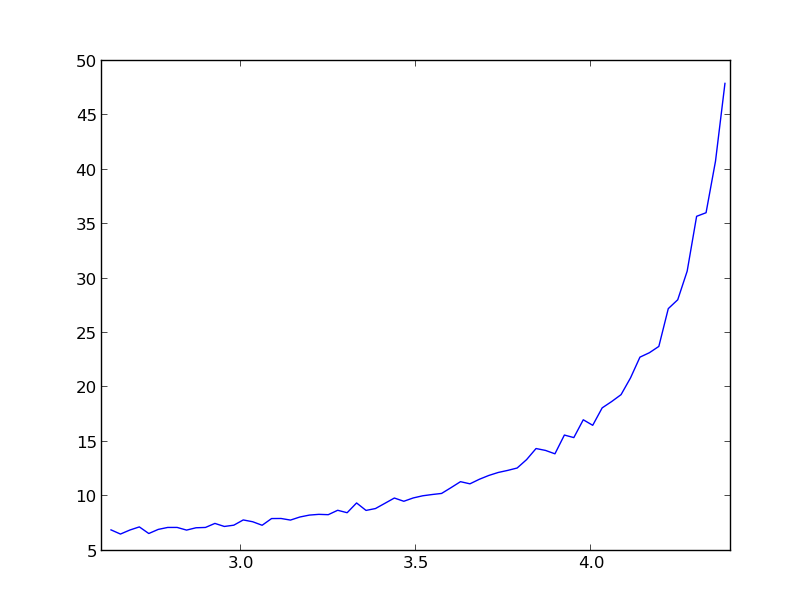
\includegraphics[width=0.9\linewidth,angle=0]{greatd.png}
\caption{Yukawa differential cross section vs. d, E=0.705,d big}
\label{figure13}
\end{center}
\end{figure}

Here is the diagram when d starts from a small value: ~\ref{figure14}

\begin{figure}
\begin{center}
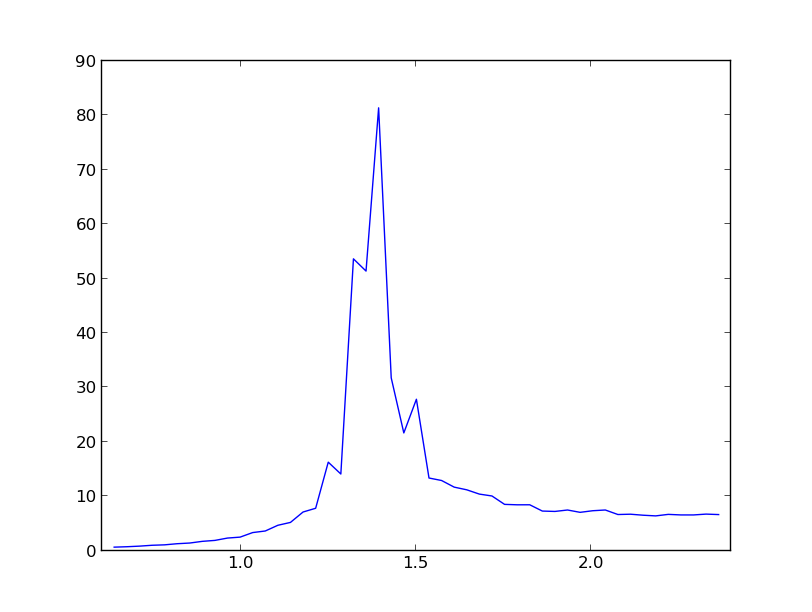
\includegraphics[width=0.9\linewidth,angle=0]{smalld.png}
\caption{Yukawa differential cross section vs. d, E=0.705,d small}
\label{figure14}
\end{center}
\end{figure}


Here is the diagram when d starts from a small value but $r_0$ very large: ~\ref{figure16}

\begin{figure}
\begin{center}
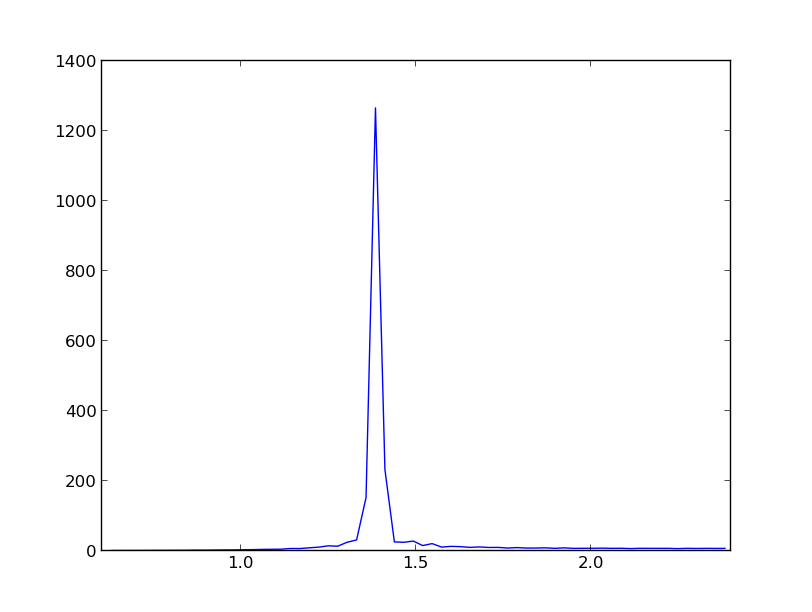
\includegraphics[width=0.9\linewidth,angle=0]{r0big.png}
\caption{Yukawa differential cross section vs. d, E=0.705,d small, $r_0$ big}
\label{figure16}
\end{center}
\end{figure}


Here is the diagram of Rutherford: ~\ref{figure15}

\begin{figure}
\begin{center}
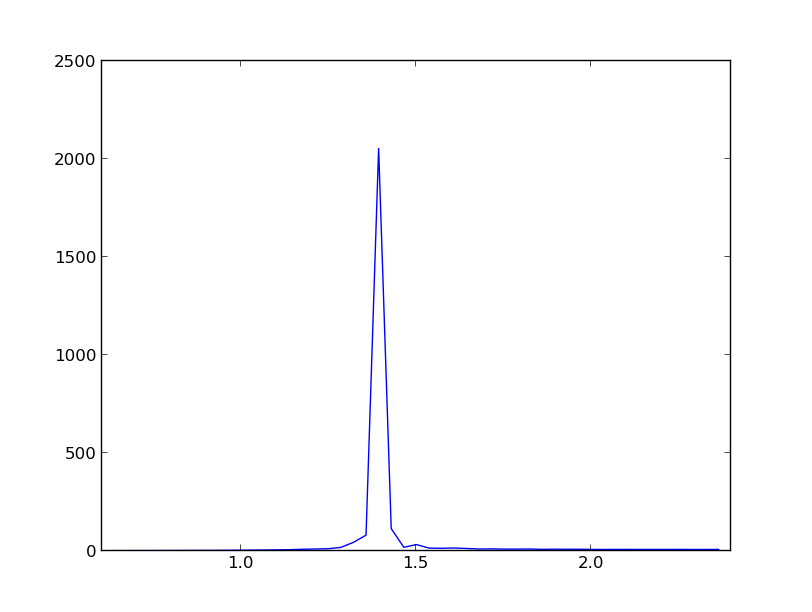
\includegraphics[width=0.9\linewidth,angle=0]{r.png}
\caption{Rutherford}
\label{figure15}
\end{center}
\end{figure}




From above we can see for large $r_0$ Yukawa scattering behaves like Rutherford, with $r_0$ increases, the more it approaches. Additionally when d start from a big value the curve behaviour approaches square law. 



\newpage
\section*{Acknowledgements}

I discussed this assignment with my classmates and used material from the
cited references, but this writeup is my own.



\newpage
\appendix
\section{Appendix}

\subsection{python code}

The following python code was used to obtain the results in this report:

\lstinputlisting[language=python]{run_root_finding.py}

\lstinputlisting[language=python]{scattering_diff.py}

\lstinputlisting[language=python]{trajectoryall.py}

\end{document}
